% 例 3：两正方形共顶点 A，BE=DG 且 BE⊥DG（手拉手特例）
\documentclass[tikz,border=4pt]{standalone}
\usepackage{ctex}
\usepackage{amsmath}
\usetikzlibrary{calc}
\begin{document}
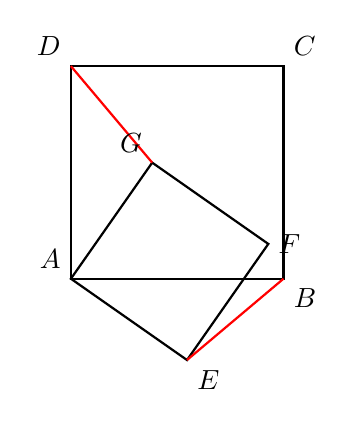
\begin{tikzpicture}[scale=0.9, thick]
  % 正方形 ABCD：A 原点；B 右、D 上
  \coordinate (A) at (0,0);
  \coordinate (B) at (3,0);
  \coordinate (C) at (3,3);
  \coordinate (D) at (0,3);
  \draw (A)--(B)--(C)--(D)--cycle;

  % 正方形 AEFG：绕 A 旋转 -35° 的小正方形，边长 2
  \def\ang{-35}
  \coordinate (E) at ({2*cos(\ang)}, {2*sin(\ang)});
  \coordinate (F) at ({2*cos(\ang)+2*cos(\ang+90)}, {2*sin(\ang)+2*sin(\ang+90)});
  \coordinate (G) at ({2*cos(\ang+90)}, {2*sin(\ang+90)});
  \draw (A)--(E)--(F)--(G)--cycle;

  % 拉手线段 BE 与 DG
  \draw[red, thick] (B)--(E);
  \draw[red, thick] (D)--(G);

  \node[above left]  at (A) {$A$};
  \node[below right] at (B) {$B$};
  \node[above right] at (C) {$C$};
  \node[above left]  at (D) {$D$};
  \node[below right] at (E) {$E$};
  \node[right]       at (F) {$F$};
  \node[above left]  at (G) {$G$};
\end{tikzpicture}
\end{document}
